\section{Durchführung}
\label{sec:Durchführung}

Der Versuchsaufbau ist in \autoref{fig:versuchsaufbau} zu sehen.
Die Spektrallampe erzeugt Licht, das von der Kondensatorlinse gebündelt wird und auf die Spaltblende fällt.
Die Spaltblendenöffnung wirft ein Bild der Spaltblende auf den Eintrittsspalt, das Geradsichtprisma trennt die emittierten Spektrallinien räumlich.
Das Schutzgehäuse und somit die Photozelle selbst ist schwenkbar, sodass Licht mit verschiedenen Wellenlängen untersucht werden kann.

\begin{figure}
    \centering
    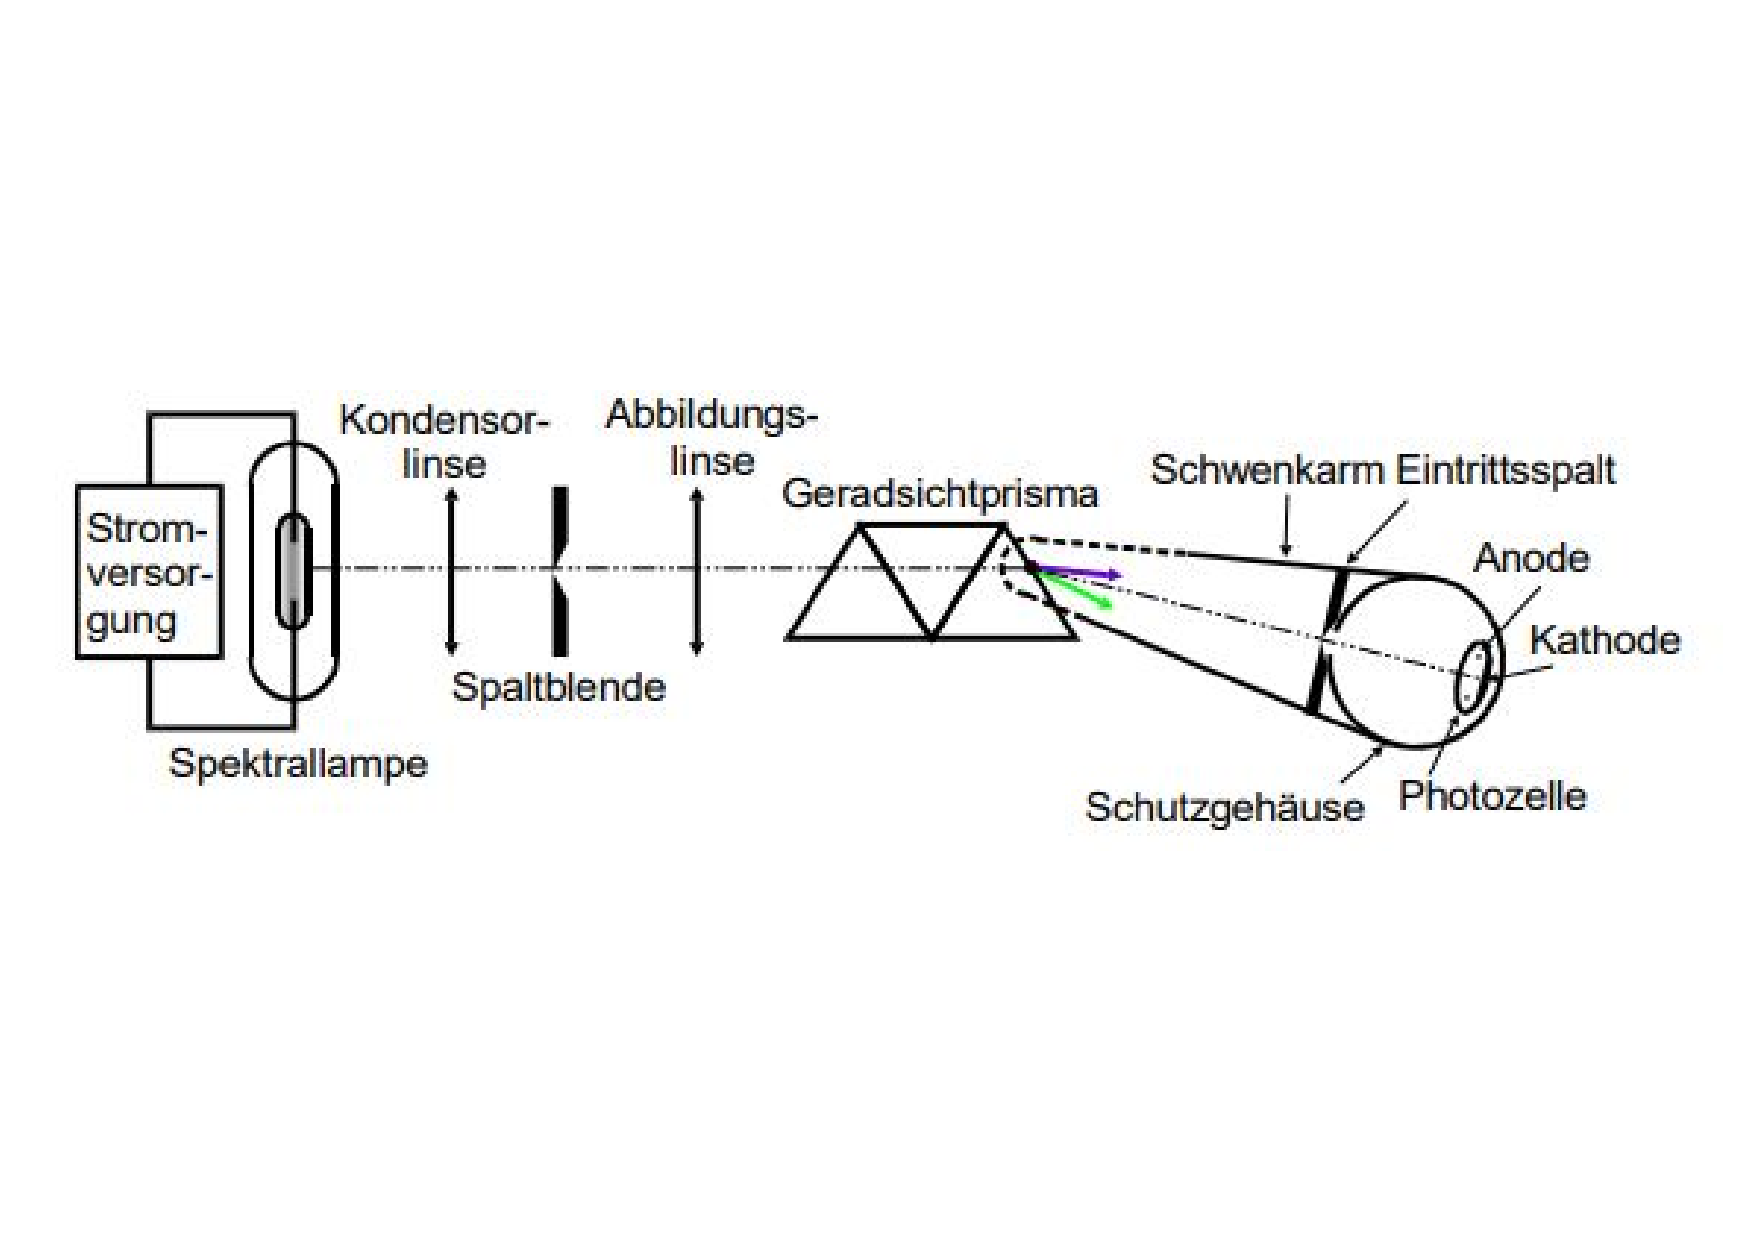
\includegraphics[width =\textwidth]{content/versuchsaufbau.pdf}
    \caption{Versuchsaufbau zur Untersuchung des Photoeffekts.\cite{anleitung}}
    \label{fig:versuchsaufbau}
\end{figure}
\noindent
Bei der verwendeten Spektrallampe handelt es sich um eine Quecksilberlampe.
Zunächst werden die Linsen und die Spaltblende so eingestellt, dass die Spektrallinien so breit wie der Eintrittsspalt und scharf genug sind.
Den Versuchsaufbau vor Ort ist in \autoref{fig:aufbau} zu sehen.
Die zu untersuchenden Farben sind in \autoref{fig:farben} zu finden.
Folgende Farblinien werden untersucht: rot, gelb, grün und violett.

\noindent
Dabei wird das Schutzgehäuse der Photozelle so bewegt, dass der Eintrittsspalt vollständig von der Spektrallinie bestrahlt wurde.
In gleichmäßigen Abständen wird die Gegenspannung $U$ von $\SI{5}{\volt}$ auf $\SI{-5}{\volt}$ verändert, wobei um $\SI{0}{\volt}$ kleinschrittiger vorgegangen wird.
Die Werte des Photostroms $I$ werden in Abhängigkeit von der Gegenspannung $U$ notiert.
Analog werden die anderen Spektrallinien untersucht, bei der gelben Linie soll die Gegenspannung von $\SI{20}{\volt}$ bis $\SI{-20}{\volt}$ laufen.

\begin{figure}
    \centering
    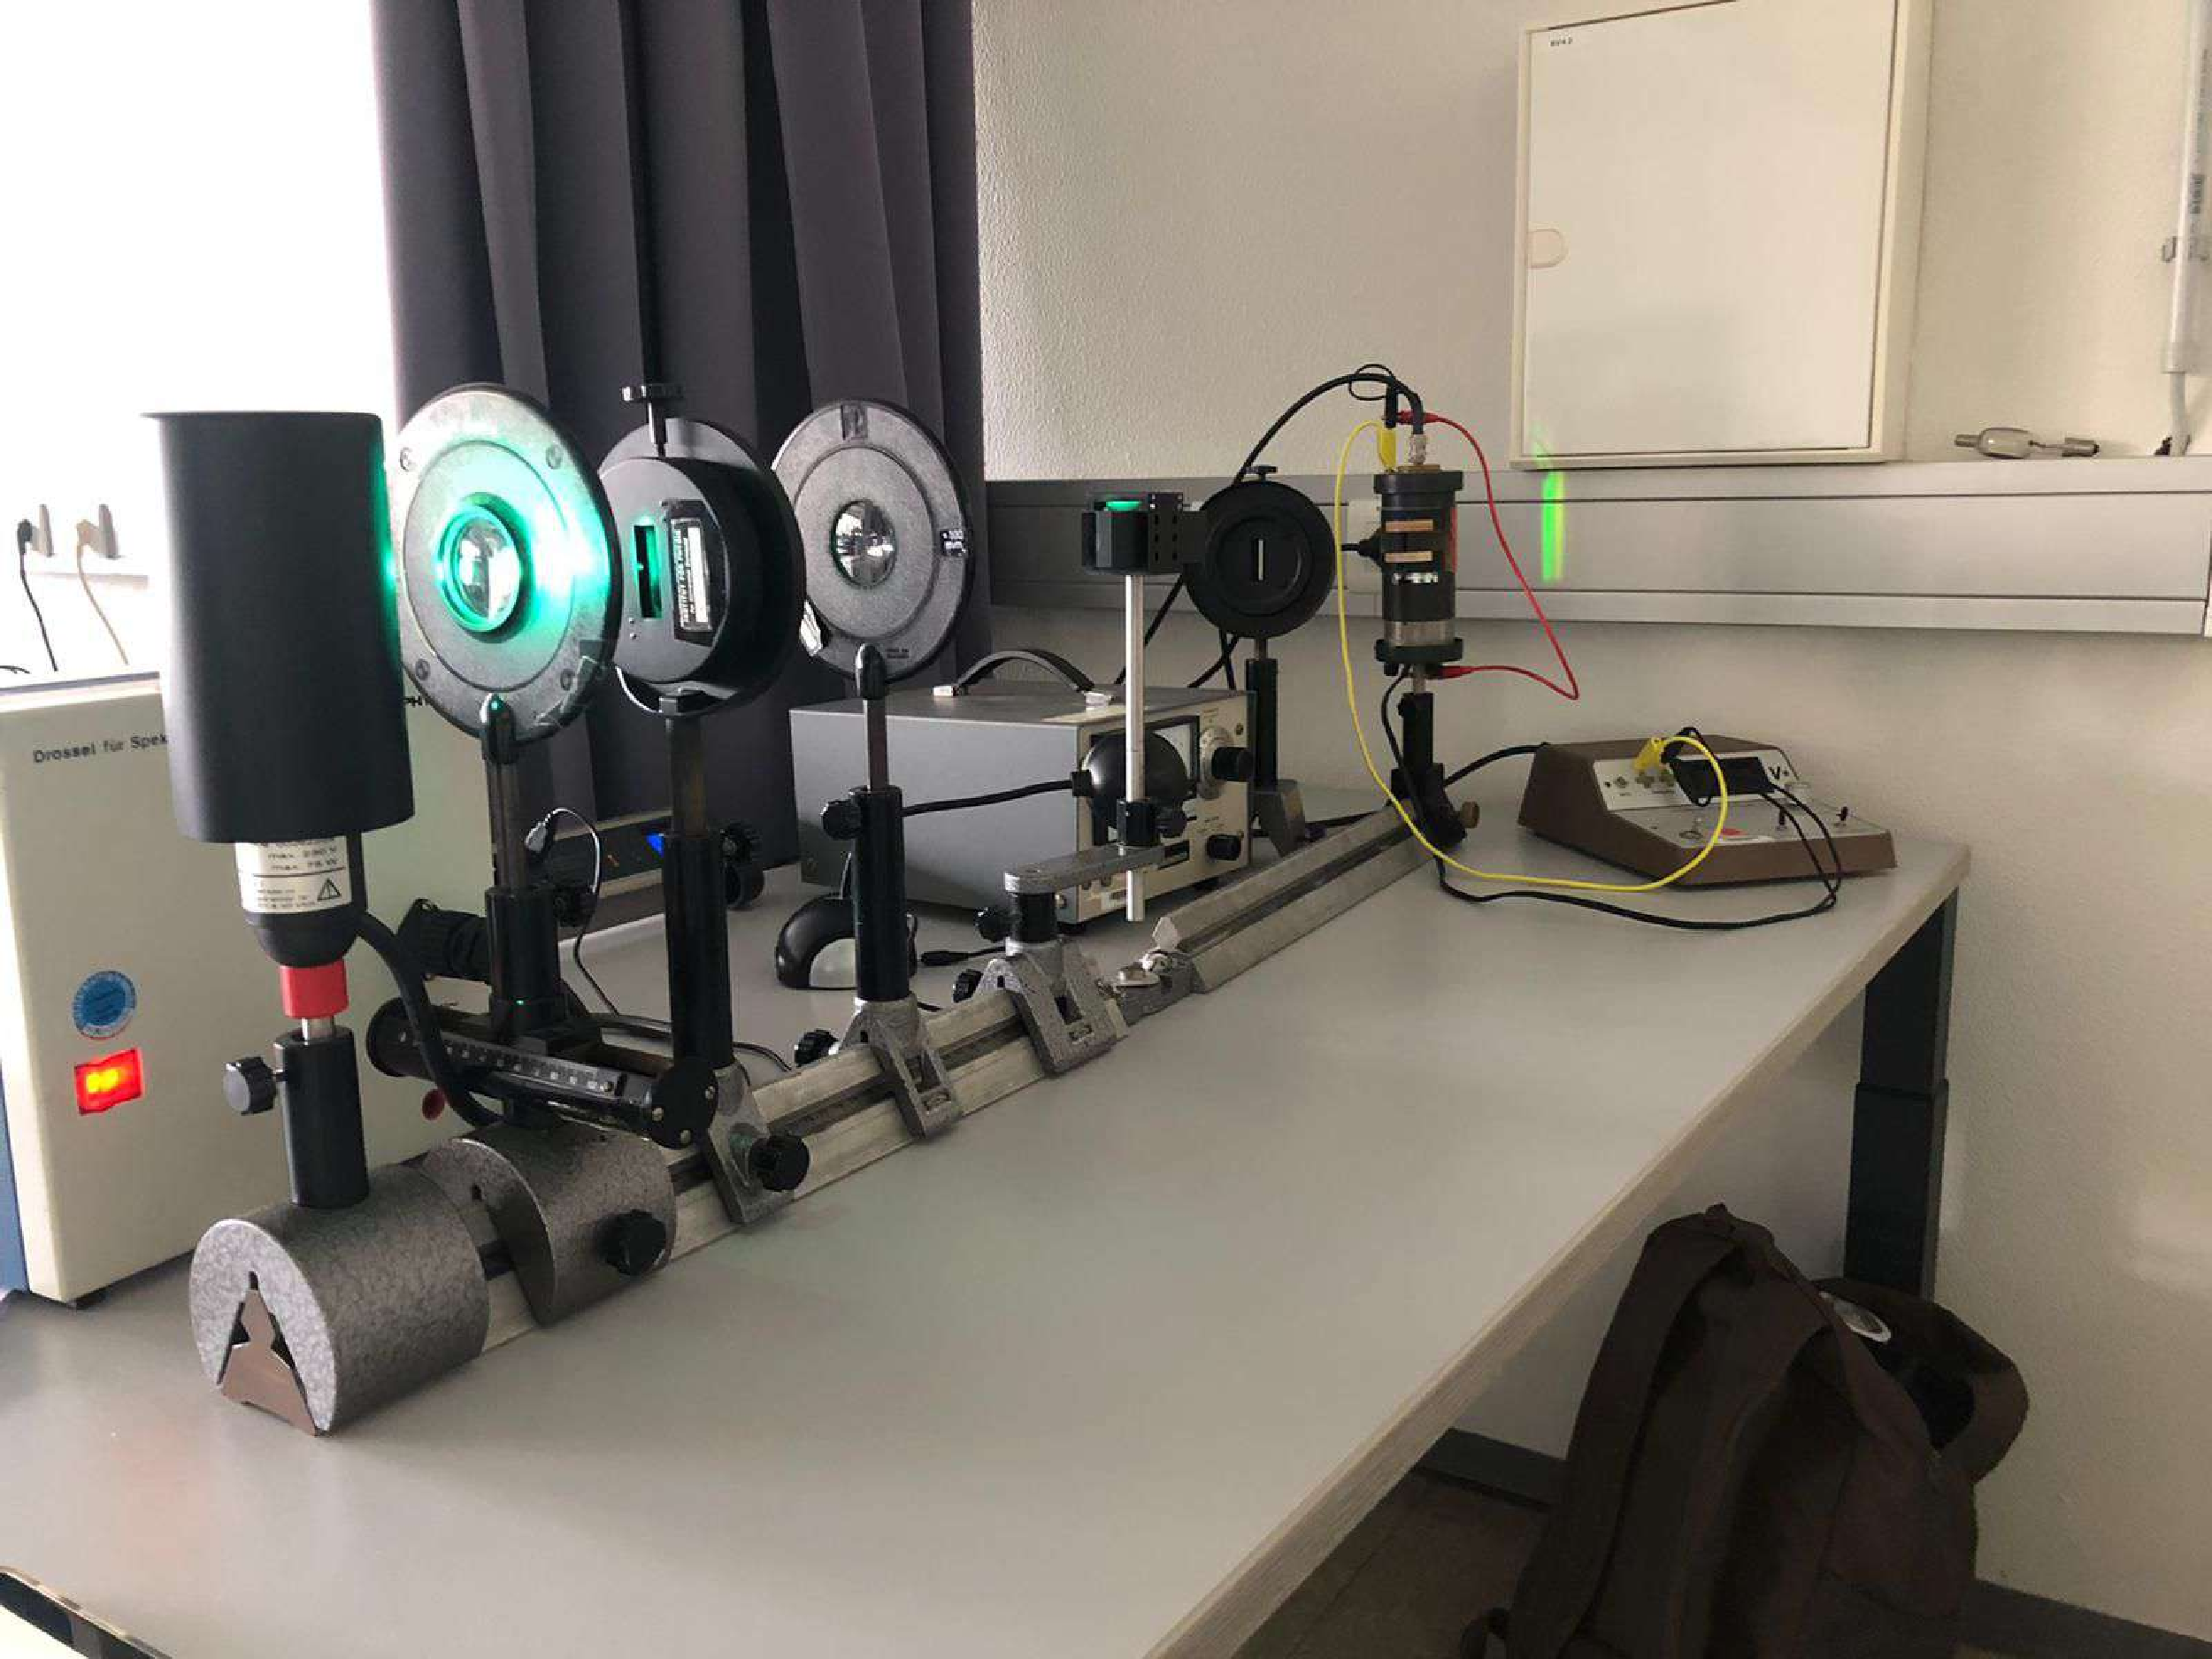
\includegraphics[width =\textwidth]{content/aufbaufotot.pdf}
    \caption{Versuchsaufbau vor Ort. Links ist die Hg-Dampflampe zu sehen, auf der Schiene folgen dann von links nach rechts eine Linse, ein Spalt, und eine weitere Linse.
    Anschließend folgt ein Prisma, welches das Licht aufspaltet.
    Auf einem weiteren Schienenteil, welches sich auf einem Kreisbogen relativ zu dem anderen Teil bewegen lässt, befindet sich die Photozelle.
    Hinter dem Stab, der das Prisma trägt, ist das Pico-Amperemeter zu sehen.
    Das bräunliche Gerät, aus dem das gelbe Kabel kommt, ist der Generator für die Gegenspannung.}
    \label{fig:aufbau}
\end{figure}

\begin{figure}
    \centering
    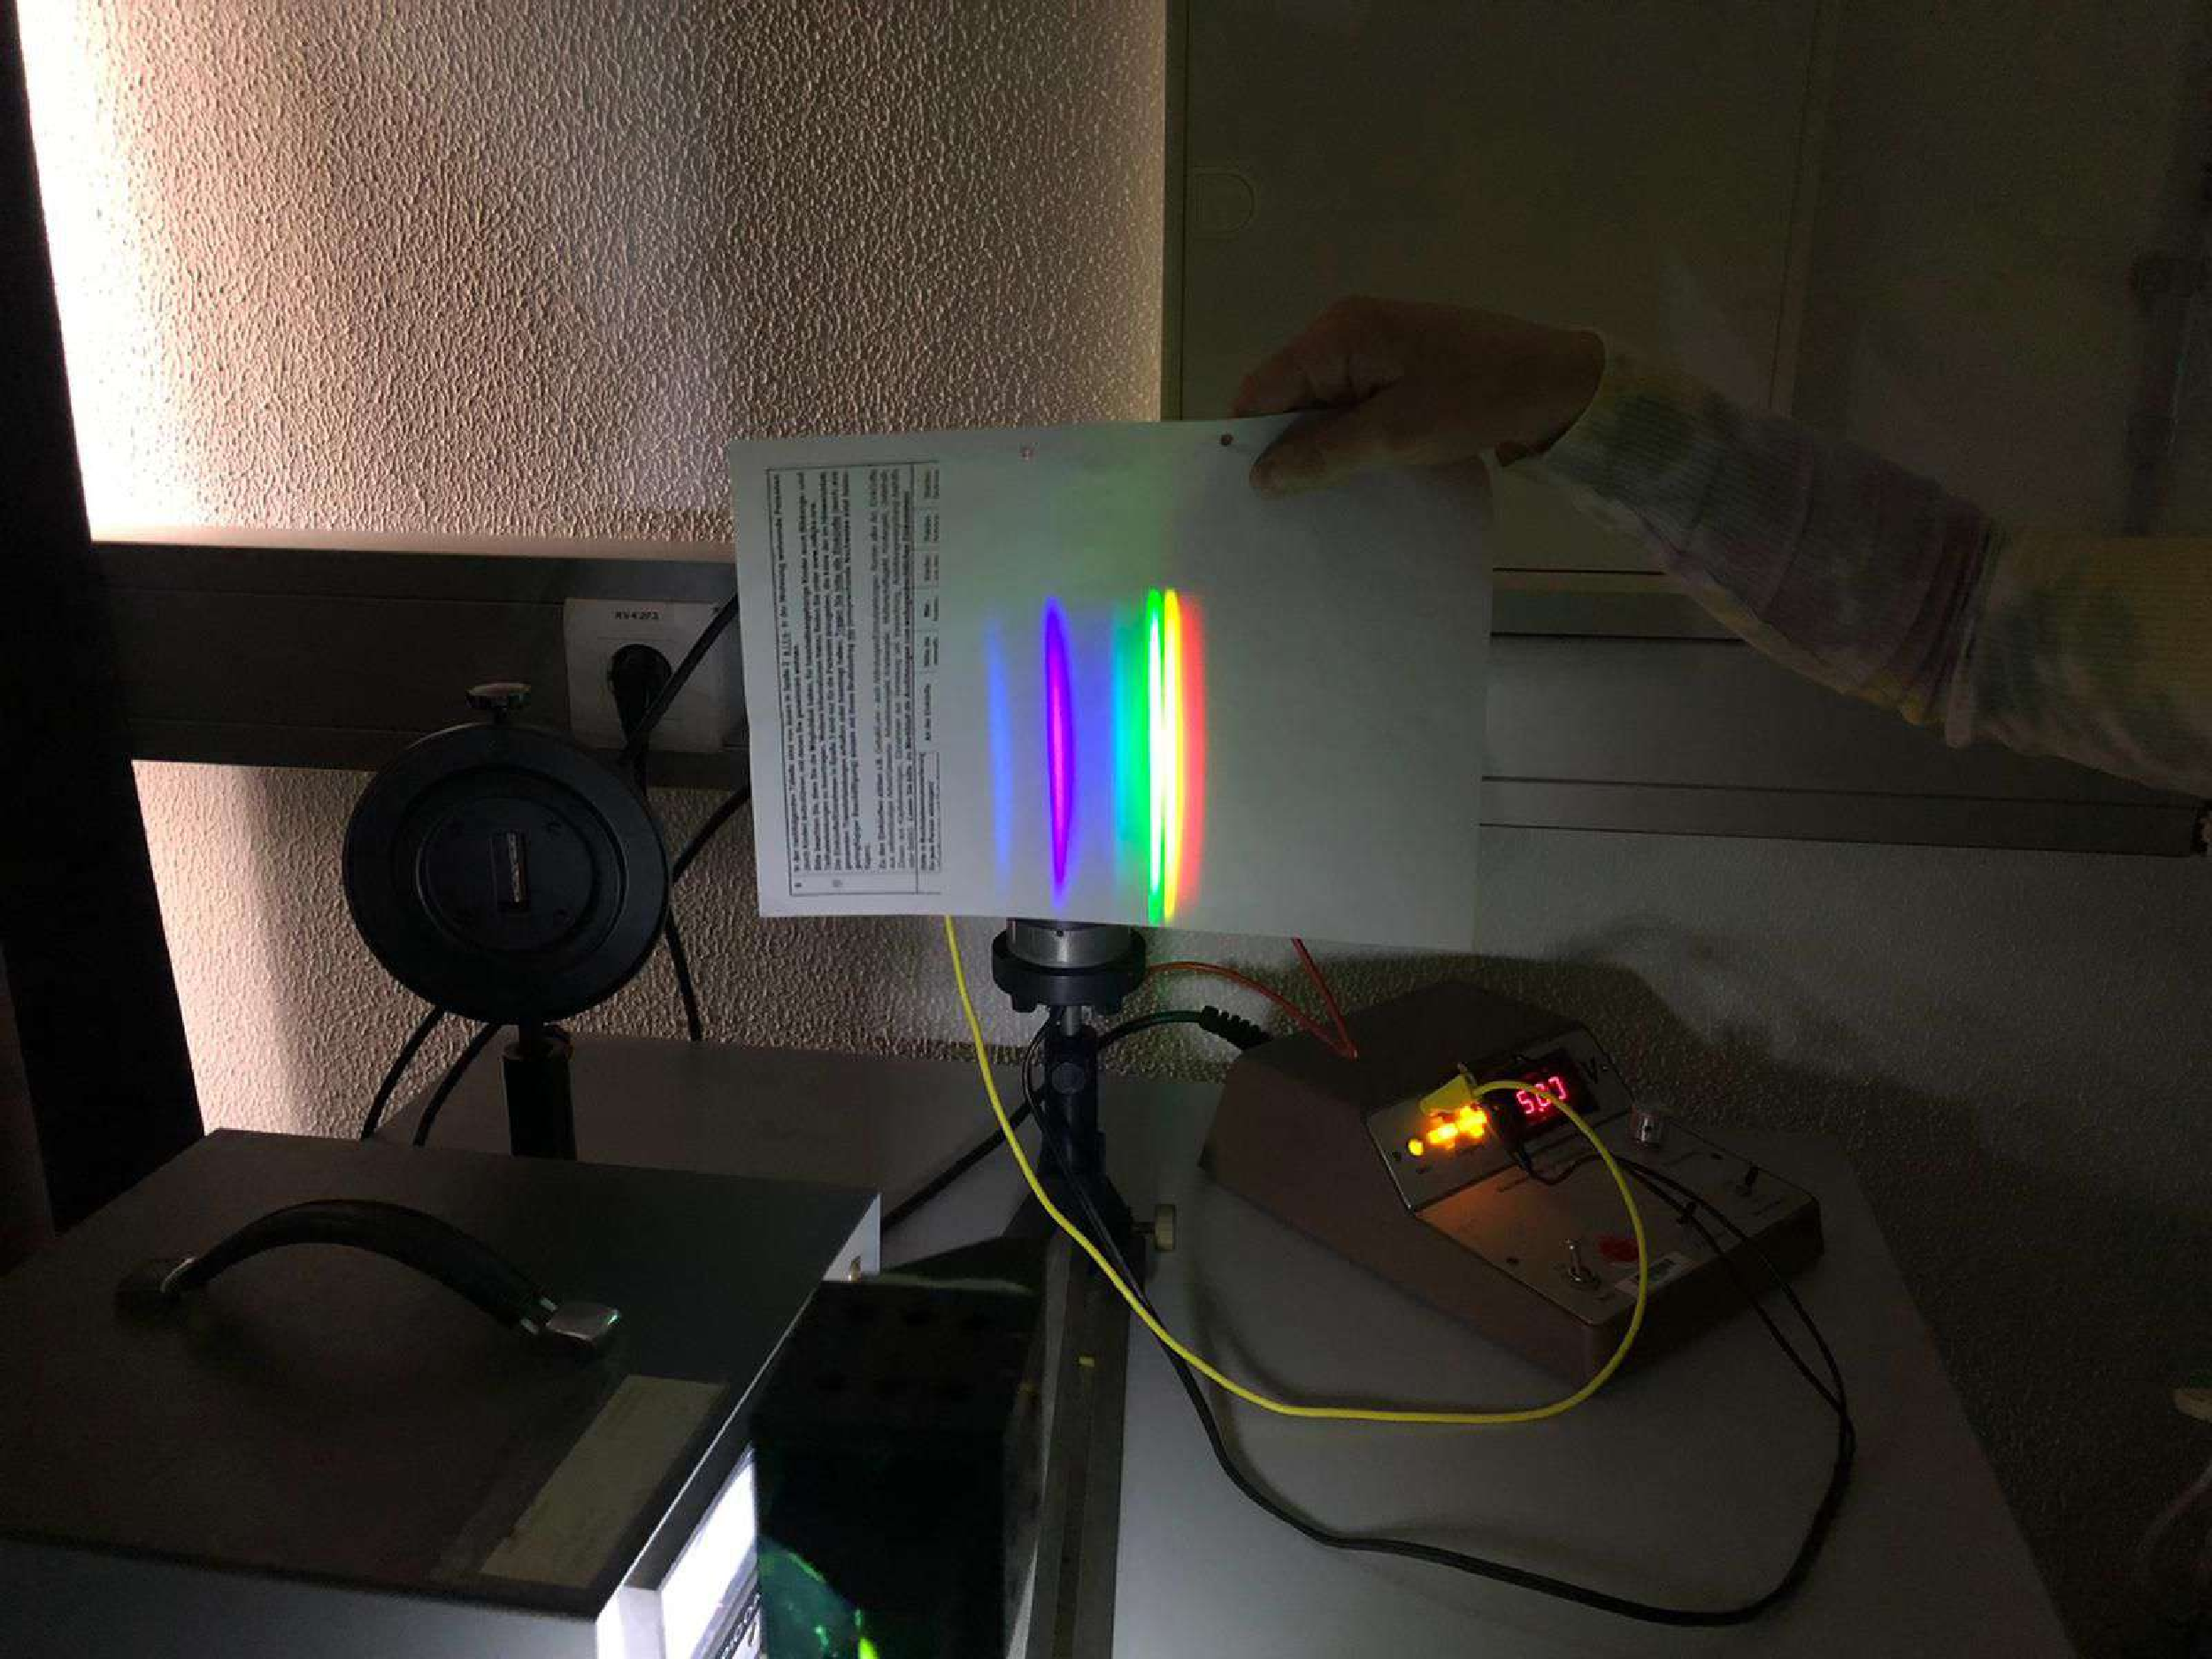
\includegraphics[width =\textwidth]{content/farben.pdf}
    \caption{Spektrallinien.}
    \label{fig:farben}
\end{figure}